\documentclass[12pt,a4paper]{report}
\usepackage{graphicx}
\usepackage{lipsum}% http://ctan.org/pkg/lipsum
\usepackage{titletoc}% http://ctan.org/pkg/titletoc
\usepackage[T1]{fontenc}
\usepackage{natbib}
\usepackage{url}
\usepackage{titlesec}
\usepackage{graphicx}

\usepackage{enumitem}

\usepackage{layout}
\setlength{\voffset}{-0.5in}
\setlength{\headsep}{5pt}


\newenvironment{tightcenter}{%
  \setlength\topsep{0pt}
  \setlength\parskip{0pt}
  \begin{center}
}{%
  \end{center}
}

\usepackage{float}
\graphicspath{ {images/} }
\tolerance=1
\emergencystretch=\maxdimen
\hyphenpenalty=10000
\hbadness=10000  
\titleformat{\chapter}{\normalfont\huge}{\thechapter.}{20pt}{\huge}
\titlespacing*{\chapter}{0pt}{0pt}{20pt}


\begin{document}
\begin{titlepage}
	\centering
	{\scshape\LARGE University of Bath \par}
	\vspace{1cm}
	{\scshape\Large Project Proposal\par}
	\vspace{1.5cm}
	{\huge\bfseries Development of a Serious Game to teach Aristotle's Syllogisms\par}
	\vspace{2cm}
	{\Large\itshape James Treasure\par}
	\vfill
	supervised by\par
	Dr.~Willem \textsc{Heijltjes}
	\vfill
	{\large \today\par}
\end{titlepage}

\tableofcontents
\chapter{Problem Description}
The younger generation of today have grown up in a world consumed in technology. \cite{oblinger2005educating} described them as the \textit{Net Generation}, the generation who always need to be connected, require immediate feedback and crave social interaction. The research of \cite{prensky2001games} explains how this vast amount of technology now experienced in everyday life has led to these newer generations having their minds rewired. These cognitive changes have caused a different set of educational preferences when compared to previous generations, with teaching methods not evolving in order to take this in to account.

Serious Games are a movement within the game industry comprised of software developers and researchers who are using games to tackle this problem. Whilst there is some debate around what exactly construes a serious game, \cite{michael2005serious} define one as any game where entertainment is not the primary purpose, but where instead the focus is on education. 

One of the benefits of using games to teach is their accessibility. In the United Kingdom  access to the internet has doubled over the past 10 years, with 82\% of adults now using the internet on a daily basis \citep{onssurvey}. With such a high number of people using the internet it allows games hosted on the web to be available to the masses. Games also appeal to a wide audience by crossing demographic boundaries such as age, gender and educational status \citep{griffiths2002educational}. 

As discussed by \cite{malone1981toward} games are also intrinsically motivating, such that there are no external factors as to why a person is playing other than for their own enjoyment. By carrying this intrinsic motivation into serious games, it is clear that this could be used to engage people who otherwise might not have been interested in learning. 

Formative and summative assessments are two common ways that feedback is delivered to students in education. Whereas formative assessments are carried out during the learning process, summative assessments tend to take place at the end of it. As explained by \cite{irons2007enhancing}, formative assessments can be hugely beneficial as they enhance the learning process by creating a positive environment which in turns results in greater motivation for learning. 

Serious Games lend themselves extremely well to delivering formative feedback to players through in-game features such as progress bars, score count and countdown timers. Feedback can also be provided to the player as they make mistakes allowing the player to engage with the game and keep on track to completing their goals. This can also help the player from becoming frustrated and not able to progress past a certain point.


\section{Aim}
Design and develop a web based game to teach the player about Aristotle's Syllogisms.
Syllogisms have been chosen to be turned into a game for a number of reasons. Firstly, syllogisms have had a huge cultural significance on the history of logic in the western world \citep{sep-aristotle-logic}. Aristotle's work on logic was the earliest known formal study of the the topic, which was not replaced in academia until the 19th century with Gotlobb Frege's first order logic.
Syllogisms are a very accessible way of learning about formal logic as they can depicted entirely through the use of diagrams or natural language. It can be hard to grasp the concept of other formal logic systems when examples use set theory notation and letters to represent ideas.
Using real world examples when teaching syllogisms allows the difficulty to be extracted out making the concepts far easier for the learner. Traditionally, syllogisms are represented sententially.
\bigbreak
\begin{tightcenter}
\textit{All men are mortal}\\
\textit{All Greeks are men}\\
\textit{All Greeks are mortal}\\
\end{tightcenter}
\bigbreak
However, representing syllogisms this way is not the most effective as they can be logically quite complex. As \cite{larkin1987diagram} explain, sentential form requires inferences to be made, and then those inferences to be held in memory. Throughout working through the syllogism those inferences must be continually remembered whilst working through the problem.


There are a number of graphical notations that aim to remedy this problem. The most common representation is in the form of Venn diagrams, but alternatives such as Euler and Linear diagrams both exist.


This game will use the Venn diagram representation to depict syllogisms.
There will be multiple levels with the difficulty progressing with each one. Initially as little mathematical notation as possible will be used, with set theory notations being introduced as the complexity increases. The game will initially begin with a small section teaching the basics of Venn Diagrams as these will be need to be understood in order to play. Completion of the game will result in the user being able to recognise and differentiate different examples of syllogisms. User tests will then be carried out to assess the effectiveness of the game as a method for teaching syllogisms.

\section{Objectives}
\begin{itemize}
  \item Investigate existing Serious Games, with particular focus on teaching concepts related to Mathematics and logic.

  \item Design, develop and release a Serious Game that can be used to teach the concepts laid out in Aristotle's Syllogism.
  
  \item Ensure that the game is accessible regardless of players initial understanding of the subject.
  \item Evaluate the effectiveness of the game on users.
  
\end{itemize}

\chapter{Requirements Specification}
   \section{Functional}
   \begin{enumerate}[label*=\thesection .\arabic*]
            \item The game will be written using HTML, CSS and JavaScript. The HTML5 element, Canvas, will be used to animate the game.\\
            \textit{These are the current standards for web development. Canvas is chosen over SVG as Canvas can be written in pure JavaScript. Canvas also has better performance than SVG, although that likely will not be a concern with a game of this nature. }
            \item There must be an initial prototype of the game.\\
            \textit{This is not only important as there is a progress demonstration that must be carried out but as it will provide an opportunity to gather feedback on the current state of the game.}
            \item The game must run on all common browsers.\\
            \textit{There are a number of known issues with some Canvas features on certain browsers. It is important to have a consistent experience across all browsers to not detract from the experience of playing the game. }
            \item The game must have multiple levels.\\
            \textit{This allows the game to progress in difficulty, allowing the player to learn more advanced aspects of syllogisms.}
            \item The game will be played using the mouse.\\
            \textit{By allowing only the mouse to used to play the game it will make it compatible with devices that do not have a keyboard.}
            \item The game must successfully recognise when the player has completed a level.\\
            {By not recognising potential end game scenarios it could confuse the player in to thinking they are incorrect. This would lead to reduced engagement with the game.}
        \end{enumerate}
   \section{Non-functional}
   \begin{enumerate}[label*=\thesection.\arabic*]
            \item The game should be playable on tablets and mobile phones.\\
            \textit{Having all controls for the game on screen and using no keyboard input will allow the game to be played across all devices. This aids accessibility as players may not have access to a traditional PC.}
            \item The game must have an elegant user interface.\\
            \textit{It is important to not crowd the users with an excessive number of buttons and options in the game. As no keyboard controls will be used, the challenge will be to provide a way to operate all controls of the game efficiently.}
             \item The game must feature a tutorial at the beginning.\\
            \textit{A tutorial is crucial to explain the premise and controls of the game. Not including a tutorial would leave the player confused and unsure of how to play. }
             \item The game should run at 60 frames per second.\\
            \textit{Games at 60 frams per second appear much smoother to the player. This keeps focus on the game and not on the graphics.}
        \end{enumerate}



\chapter{Project Plan}
\noindent 
The project has four specific milestones with hard deadlines, that have been broken down to show a more granular view of the work that needs to be completed. The Gantt Chart in Figure~\ref{fig:ganntchart} shows how long will be spent on each milestone.
\section{Milestones}
\begin{enumerate}
  \item Project Proposal
  \item Literature Review
  \begin{itemize}
  \item Research
  \item Write review
  \end{itemize}
  \item Development
  \begin{itemize}
  \item System Design
  \item Prototype Development
  \item System Development
  \item System Testing
  \item User Testing
  \end{itemize}
  \item Write Dissertation
\end{enumerate}

\begin{figure}[h]
\caption{Gannt Chart}
\centering
\label{fig:ganntchart}
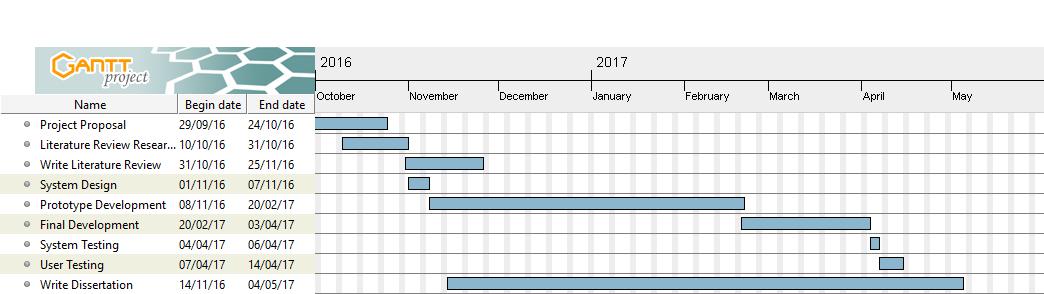
\includegraphics[width=\textwidth,height=\textheight,keepaspectratio]{Gantt}
\end{figure}



{\let\clearpage\relax\chapter{Resources}}
\section{Software Resources}
HTML, CSS and JavaScript will be used to implement the game are all freely available. WebStorm, a web development IDE, will be used to develop the game.

\section{Hardware Resources}
A PC will be needed to carry out the software development and dissertation write up of the project. A server will also be needed to host the game.

\section{Human Resources}
Users will be required to test the game and give their feedback. 
Meeting time with supervisor (Dr.~Willem Heijltjes) will be needed to discuss progress and direction of the project.

\bibliographystyle{plainnat}
\bibliography{bibliography} 

\end{document}
